\documentclass[a4paper, notitlepage]{report}

%====================== PACKAGES ======================

\usepackage[english]{babel}
\usepackage[utf8]{inputenc}

\usepackage[sorting=none]{biblatex}
\usepackage{csquotes}
\bibliography{bibliographie}


%pour gérer les positionnement d'images
\usepackage{float}
\usepackage{amsmath}
\usepackage{graphicx}
\usepackage{braket}
\usepackage[colorinlistoftodos]{todonotes}

\usepackage{xcolor}
\definecolor{ups}{RGB}{86,08,59}
\definecolor{cs}{RGB}{148,13,56}

\usepackage{url}
%pour les informations sur un document compilé en PDF et les liens externes / internes
\usepackage{hyperref}
\hypersetup{%
  colorlinks=false,% hyperlinks will be black
  linkbordercolor=cs,% hyperlink borders will be red
  urlbordercolor=cs,% hyperlink borders will be red
  citebordercolor=cs,
%   pdfborderstyle={/S/U/W 1}% border style will be underline of width 1pt
}
%pour la mise en page des tableaux
\usepackage{array}
\usepackage{tabularx}
%espacement entre les lignes
\usepackage{setspace}
\usepackage{svg}

\usepackage{wrapfig}
\usepackage{multicol}

% Special symbols
\usepackage{amssymb}
\usepackage{mathrsfs}

%police et mise en page (marges) du document
\usepackage[T1]{fontenc}
\usepackage[top=2cm, bottom=2cm, left=2cm, right=2cm]{geometry}
%Pour les galerie d'images
\usepackage{subfig}
\usepackage{tikz}
\usetikzlibrary{positioning}
\usetikzlibrary{calc}
\usepackage{tikz-cd}

% Algorithms
\usepackage{algorithm}
\usepackage{algpseudocode}
\usepackage{listings}
\renewcommand\lstlistingname{Programme}
\renewcommand\lstlistlistingname{Liste des programmes}
\definecolor{codegreen}{rgb}{0,0.6,0}
\definecolor{codegray}{rgb}{0.5,0.5,0.5}
\definecolor{codepurple}{rgb}{0.58,0,0.82}
\definecolor{backcolour}{rgb}{0.95,0.95,0.92}
\lstdefinestyle{mystyle}{
    commentstyle=\color{ups},
    keywordstyle=\color{cs},
    numberstyle=\tiny\color{codegray},
    stringstyle=\color{ups},
    basicstyle=\ttfamily,
    breakatwhitespace=false,
    breaklines=true,
    captionpos=b,
    keepspaces=true,
    numbersep=5pt,
    showspaces=false,
    showstringspaces=false,
    showtabs=false,
    tabsize=2
}

\lstset{style=mystyle}


% No new page after chapter
\usepackage{etoolbox}
\makeatletter
\patchcmd{\chapter}{\if@openright\cleardoublepage\else\clearpage\fi}{}{}{}
\makeatother

\newcommand{\RE}{\mathrm{Re}}
\newcommand{\IM}{\mathrm{Im}}
\newcommand{\function}[5]{\begin{array}{l|rcl}
#1: & #2 & \longrightarrow & #3 \\
    & #4 & \longmapsto & #5 \end{array}}
\newcommand{\mathsc}[1]{{\normalfont\textsc{#1}}}
\newcommand*{\toccontents}{\@starttoc{toc}}

%====================== INFORMATION ET REGLES ======================

%rajouter les numérotation pour les \paragraphe et \subparagraphe
\setcounter{secnumdepth}{4}
\setcounter{tocdepth}{4}



%======================== DEBUT DU DOCUMENT ========================

\begin{document}

%régler l'espacement entre les lignes
\newcommand{\HRule}{\rule{\linewidth}{0.5mm}}

%page de garde
\begin{center}

% Upper part of the page. The '~' is needed because only works if a paragraph has started.
\includesvg[width=\textwidth]{./figures/Logo}~\\[1cm]

% \textsc{\LARGE CentraleSupélec}\\[1.5cm]

\textsc{\Large }\\[0.5cm]

% Title
\HRule \\[0.4cm]

{\huge \bfseries Autour des Diagrammes de Décision Quantiques\\
[0.4cm] }

{\large \bfseries Rapport -- Parcours recherche -- Projet S7\\[0.4cm] }
{\large \bfseries \textsl{Élève : Malo \textsc{Leroy}}\\ }
{\large \bfseries \textsl{Encadrant : Renaud \textsc{Vilmart}}\\[0.4cm] }


\HRule \\[1.5cm]

\begingroup
\let\clearpage\relax
\tableofcontents
\endgroup

\vfill

% Bottom of the page
{\large {17 février 2025}}

\end{center}

%page blanche
%\newpage
%~
%ne pas numéroter cette page
\thispagestyle{empty}


\thispagestyle{empty}
\setcounter{page}{0}
%ne pas numéroter le sommaire

%\newpage

%espacement entre les lignes d'un tableau
\renewcommand{\arraystretch}{1.5}

%====================== INCLUSION DES PARTIES ======================

~
\thispagestyle{empty}
%recommencer la numérotation des pages à "1"
\setcounter{page}{0}
\newpage

\chapter{Introduction} % 1 page max
\label{ch:Introduction}


\section{Contexte et objectif}
\label{sec:Contexte}

L'\textbf{informatique quantique} est un domaine en plein essor. Cette technologie permettant de manipuler des qubits à la place des bits qui sont à la base de l'informatique actuelle, ouvrent la voie à des algorithmes plus performants que les algorithmes classiques. Les machines quantiques exécutant ces algorithmes étant encore en développement et d'un coût important, il existe un besoin d'outils de simulation et de vérification d'algorithmes quantiques par des machines classiques. L'objectif de ce projet est de proposer un modèle sur les diagrammes de décision quantiques, en s'appuyant sur les travaux existants, et de les simuler pour en étudier les performances.

\section{État de l’art}
\label{sec:Etat}

\subsubsection*{Informatique quantique}

Le premier postulat de la physique quantique, le \textbf{principe de superposition}, énonce que l'espace des états d'un système quantique est un espace de Hilbert. Par conséquent, si un \textit{bit} ne peut classiquement être que dans un état $\ket 0$ ou $\ket 1$, son homologue quantique le \textbf{qubit} peut être dans une superposition de ces deux états.
$$\ket \psi = \alpha \ket 0 + \beta \ket 1$$

Où $\alpha, \beta$ sont des coefficients complexes. Le second postulat, le \textit{principe de mesure}, stipule que lorsqu'un qubit est mesuré, il est projeté sur un des états de base $\ket 0$ ou $\ket 1$ avec une probabilité $|\alpha|^2$ ou $|\beta|^2$ respectivement.

Les états à $n$ qubits sont peuvent être représentés par des \textbf{vecteurs} de dimension $2^n$, les états de l'ensemble constitué de deux systèmes étant ceux obtenus par produit tensoriel (\textit{produit de Kronecker}) d'un état du premier système et d'un état du second. C'est ce nombre exponentiel de paramètres complexes pour un état à plusieurs qubits rend l'étude classique d'algorithmes quantiques difficile, puisque les états prennent une taille exponentiellement grande en mémoire.

\subsubsection*{Diagrammes de décision}

La structure de \textbf{diagramme de décision} est une structure de données développée à partir des années 1970. Elle est depuis devenue largement utilisée en informatique, notamment pour rendre plus compacte la représentation de \textbf{fonctions binaires} \cite{Minato_1996}.

Prenons par exemple la fonction $f(x_1, x_2, x_3) = x_1 \lor (x_2 \land x_3)$. La représentation d'une telle fonction se fait dans le cas général à l'aide d'une \textit{table de vérité}. On peut utiliser une représentation plus compacte en utilisant un diagramme de décision, comme le montre la Figure \ref{fig:ExempleDD}, où les fils gauches sont signalés par des flèches pointillées et les fils droits sont signalés par des flèches continues.

\begin{figure}
  \renewcommand{\arraystretch}{0.8}% Tighter
  \begin{tabular}{c|c|c|c}
    $x_1$ & $x_2$ & $x_3$ & $f(x_1, x_2)$ \\
    \hline
    0 & 0 & 0 & 0 \\
    0 & 0 & 1 & 0 \\
    0 & 1 & 0 & 0 \\
    0 & 1 & 1 & 1 \\
    1 & 0 & 0 & 1 \\
    1 & 0 & 1 & 1 \\
    1 & 1 & 0 & 1 \\
    1 & 1 & 1 & 1
  \end{tabular}
  \hfill{}
  % https://tikzcd.yichuanshen.de/#N4Igdg9gJgpgziAXAbVABwnAlgFyxMJZAJgBoAGAXVJADcBDAGwFcYkQAPAfQEYACADoDGEAE58AFN2KDh9MFD7cAzAEoQAX1LpMufIRTLSy6nSat2PTdpAZseAkXIVTDFm0QgpvdVp339J1IeV3MPL2lfGzs9RxRnYlD3dm81a39Yg2QeYySLT3J0210HLJyQmjd8zi4ZIUZ5RRUimNKiMkTKsPZmjVMYKABzeCJQADNRCABbJGcQHAgkADYaRiwwcKh6OAALAaKJ6dmaBaQckAAjGAUkZTmq8O5+AF4+Kz8QQ5nEFfnFxAArKt1pttnsoCAuslPNJnoVVvQrowAAolQKeURYQY7HAHSbfX6nRAAdih1Vh7xsXyQpL+SCBIDWG3YW12+zJjy4yj4r0KH2pJJO-3ODx6XOe70oGiAA
  \begin{tikzcd}[column sep=tiny]
    (x_1) &                                                                & x_1 \lor (x_2 \land x_3) \arrow[ld, dashed] \arrow[rddd, "x_1 = 1", bend left] &   \\
    (x_2) & x_2 \land x_3 \arrow[dd, "x_2=0"', dashed] \arrow[rd, "x_2=1"] &                                                                                &   \\
    (x_3) &                                                                & x_3 \arrow[ld, "x_3 = 0", dashed] \arrow[rd, "x_3=1"]                          &   \\
          & 0                                                              &                                                                                & 1
    \end{tikzcd}
    \hfill{}
  % https://tikzcd.yichuanshen.de/#N4Igdg9gJgpgziAXAbVABwnAlgFyxMJZARgBoAGAXVJADcBDAGwFcYkQQBfU9TXfQigBMpAMzU6TVu2JceIDNjwEi5MRIYs2iEOTm8lA1aWIap2jtwP8VKMkLNb2XCTCgBzeEVAAzAE4QALZIaiA4EEiiNIxYYBZQ9HAAFm76IP5BITThSGQgAEYwYFCR5FbpAcGIUWERiCIgMXHsCcmp0fSFjAAKfMqCIH5Y7kk4aRlVNTmIACzlE0gz2XUNTfGJKSXzlYvLuZyUnEA
  \begin{tikzcd}[column sep=huge, row sep=large]
    & {} \arrow[ld, dashed] \arrow[rddd, bend left] &   \\
  {} \arrow[dd, dashed] \arrow[rd] &                                               &   \\
    & {} \arrow[ld, dashed] \arrow[rd]              &   \\
  0                                &                                               & 1
  \end{tikzcd}

  \caption{(a) Table de vérité (b) Diagramme de décision (c) Diagramme de décision sans labels}
  \label{fig:ExempleDD}
\end{figure}

Les diagrammes de décision prennent avantage de la \textbf{structure} interne de la donnée (ici, une fonction booléenne). On note d'une part que les labels ne sont pas nécessaires pour reconstituer les valeurs de prises par la fonction.

D'autre part que dans le pire des cas, c'est-à-dire celui où la fonction ne possède aucune structure permettant une réduction, la taille du diagramme de décision (son nombre de branches) vaut $2^{n+1} - 2$ ce qui comme le nombre de valeurs $2^n$ à stocker dans une table de vérité, est \textbf{exponentiel} en $n$. Dans le pire cas, les diagrammes de décision ne permettent pas d'amélioration, mais ne sont pas non plus asymptotiquement pire que les tables de vérité.

\subsubsection*{Interprétation abstraite}


L'interprétation abstraite une méthode générale consistant à traiter des propriétés de programmes informatiques en les abstrayant. Elle a été introduite par Patrick et Radhia Cousot en 1977 \cite{CousotCousot77-1}. Elle peut aussi être utilisée pour résoudre des problèmes ou calculer plus rapidement.

Étudions le problème suivant : on cherche à déterminer le signe de  l'expression -12 * 7 - 13. On pourrait calculer le résultat de cette expression, mais on peut aussi remarquer que -12 et -13 sont négatifs et que 7 est positif, d'où -12 * 7 négatif, ainsi l'expression est négative. Plus formellement, on a défini à partir des \textbf{éléments concrets} que sont -12, 7 et -13 et les remplacer par les \textbf{éléments abstraits} "positif" $\oplus$ et "négatif" $\ominus$, sur lesquels on définit les opérations de somme et de produit selon les règles bien connues.

Il existe de nombreux cas d'utilisation de l'interprétation abstraite \cite{Rosendahl_1995}, pour la compilation de programmes par exemple. Nous l'utiliserons dans ce projet pour simplifier les diagrammes de décision quantiques quitte à perdre une partie de l'information qu'ils contiennent. C'est aussi le cas pour l'exemple précédent : abstraire les éléments par leur signe ne permet pas toujours de déterminer le signe de l'expression.


\section{Contribution}
\label{sec:Contribution}

Les différents concepts présentés dans l'état de l'art permettent tous d'améliorer la vitesse de calcul ou la taille en mémoire d'une donnée. Il s'agit donc de \textbf{combiner ces concepts} dans ce projet. L'objectif du projet était donc de proposer un modèle de diagrammes de décision quantiques abstraits et additifs, et de les simuler pour en étudier les performances en comparaison d'autres modèle.

De manière préliminaire, une étude des intervalles complexes polaires a été réalisée, ce qui n'avait pas été fait jusqu'à présent.
Un \textbf{modèle} mathématique de la structure de données et de méthodes de réduction ont été formalisés, et des algorithmes de réduction ont été développés pour simplifier ces diagrammes. Une \textbf{implémentation} de ces algorithmes a été réalisée, sans se baser sur des bibliothèques existantes (mise à part pour les tests unitaires).

\section{Structure du rapport}
\label{sec:Structure}

Le Chapitre \ref{ch:Modele} présente le modèle théorique de diagrammes de décision quantiques qui a été développé, y compris les algorithmes de réduction qui accompagnent celui-ci. Ensuite, le Chapitre \ref{ch:Implementation} discute de l'implémentation réalisée. Finalement, une courte conclusion est présentée dans le Chapitre \ref{ch:Conclusion}.

Un document plus complet que ce rapport destiné à être publié et rédigé en anglais, est disponible en ligne. \cite{Leroy_2024} D'éventuels points théoriques succinctement présentés dans ce rapport et ou théorèmes dont la preuve n'est pas spécifiée sont détaillés dans ce document.



\newpage

\newpage

\chapter{Modèle théorique}
\label{ch:Modele}

Le modèle théorique proposé est celui des \textbf{diagrammes de décision quantiques additifs abstraits}.

\section{Arithmétique des intervalles}
\label{sec:ArithmetiqueIntervalles}

L'arithmétique des intervalles dans le cadre de l'interprétation abstraite est proche de l'exemple de calcul sur les signes de la \autoref{sec:Etat}. L'arithmétique des intervalles est utilisée pour déterminer un ensemble de valeurs possibles pour une expression mathématique en utilisant des intervalles pour les valeurs des variables.

L'arithmétique des intervalles réels a été étudiée \cite{Sunaga_2009}, et l'arithmétique des intervalles complexes cartésien a fait l'objet d'études légères par le passé \cite{Rokne_1971}. Au cours de ce projet, un travail a été réalisé pour explorer les possibilités de l'arithmétique des \textbf{intervalles complexes cartésiens et polaires}.

\begin{figure}
  \centering
  \resizebox{.5\textwidth}{!}{
  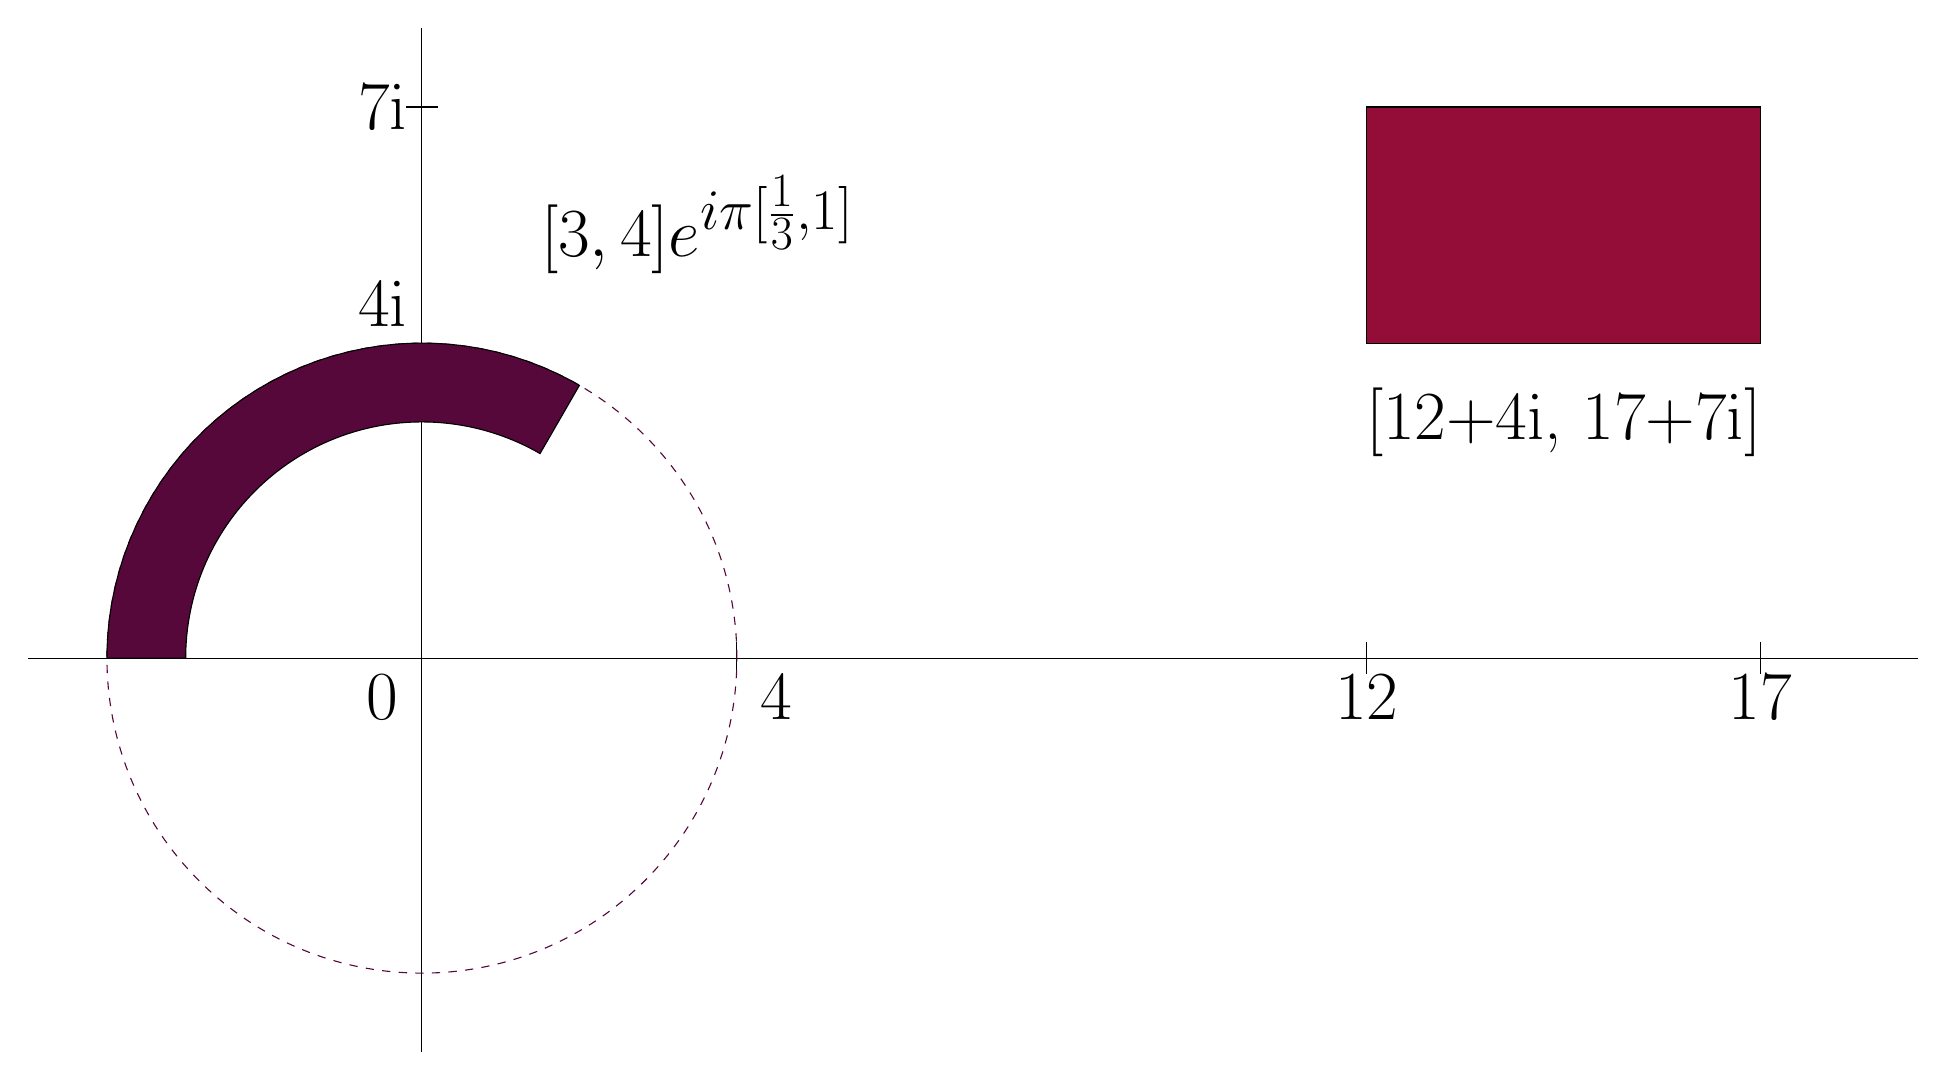
\begin{tikzpicture}
    \coordinate (c) at (0,0);
    \tikzstyle{every node}=[font=\Huge]
    \draw [fill=cs] (12,4) rectangle (17,7);
    \node at (14.5,3) {[12+4i, 17+7i]};
    \draw (-5,0) -- (19,0);
    \draw (0,-5) -- (0,8);

    \draw (4,-.2) -- (4,.2);
    \node at (4.5,-.5) {4};

    \draw (-.2,4) -- (.2,4);
    \node at (-.5, 4.5) {4i};

    \draw (-.2, 7) -- (.2, 7);
    \node at (-.5,7) {7i};

    \draw (12,-.2) -- (12,.2);
    \node at (12,-.5) {12};

    \draw (17,-.2) -- (17,.2);
    \node at (17,-.5) {17};

    \node at (-.5,-.5) {0};

    \draw [color=ups,dashed] (c) circle (4cm);
    \node at (3.5,5.5) {$[3, 4]e^{i\pi[\frac 1 3, 1]}$};
    \draw[fill=ups]
    ($(c) + (60:4cm)$) arc (60:180:4cm)
    --
    ($(c) + (180:3cm)$) arc (180:60:3cm)
    -- cycle;
  \end{tikzpicture}
  }
  \caption{Exemple d'intervalles complexes cartésiens et polaires}
  \label{fig:intervalles}
\end{figure}

Les intervalles complexes cartésiens sont définis par un intervalle pour la partie réelle et un intervalle pour la partie imaginaire. De manière équivalente, ils sont définis comme le plus petit rectangle dans le plan complexe (orienté selon les axes réel et imaginaire) contenant deux complexes. Les intervalles complexes polaires sont définis par un intervalle pour le module et un intervalle pour l'argument. Ces deux types d'intervalles ont des représentations différentes dans le plan complexe, comme le montre la \autoref{fig:intervalles}. Dans un cas comme dans l'autre, l'équivalent abstrait d'une \textbf{opération} $*$ est défini sur des éléments $\alpha$ et $\beta$ de l'ensemble des intervalles cartésiens $\mathcal{A}_0$ ou polaires $\mathcal S_0$ par
$$\alpha * \beta = \bigcap_{\gamma \supset \alpha \circledast \beta\text{ et }\gamma \in \mathcal{A}_0} \gamma \quad \text{où} \quad \alpha \circledast \beta = \{a * b ; a \in \alpha, b \in \beta\}$$

Les opérations de somme, de produit et d'union ainsi construites sont \textbf{sur-approximées} : elles garantissent que l'ensemble des valeurs possibles est inclus dans l'ensemble abstrait, et d'avoir un intervalle pour résultat. Ces opérations ont des propriétés, de distributivité par exemple, parfois très différentes des nombres complexes qu'ils représentent. Des propriétés sur les intervalles cartésiens et polaires sont énoncées et démontrées dans le document annexe \cite{Leroy_2025}.

D'un point de vue pratique, les intervalles cartésiens sont généralement plus simples à manipuler que les intervalles polaires, et sont largement plus adaptés à une structure additive. Les intervalles polaires ont des avantages pour les opérations de multiplication et de division, mais rendent la somme coûteuse en calculs et en perte de précision.

\section{États abstraits et diagrammes}

Les \textbf{états} abstraits à $n$ qubits sont définis comme des $2^n$-uplets d'intervalles complexes, on note leur ensemble $\mathcal A_n$.
Il peut s'agit des intervalles cartésiens ou polaires, puisque les opérations sont définies de manière similaire, mais en pratique on se limite souvent aux intervalles cartésiens.
On définit sur les états la relation d'ordre d'inclusion des états par l'inclusion des produits cartésiens des intervalles les composant.

Les \textbf{diagrammes} sont définis de manière récursive. Le seul diagramme de hauteur 0 est $\boxed 1$, puis si l'ensemble $\mathcal D_n$ des diagrammes de hauteur $n$ est défini, les diagrammes de hauteur $n+1$ peuvent avoir un nombre fini de fils gauches dans $\mathcal D_n$ et un nombre fini de fils droits dans $\mathcal D_n$, chacun étant associé à une amplitude abstraite sur la branche dans $\mathcal A_0$
$$\mathcal{D}_{n+1} = \mathscr{P}_f(\mathcal{A}_0 \times \mathcal{D}_n) \times \mathscr{P}_f(\mathcal{A}_0 \times \mathcal{D}_n)$$

On peut ainsi définir la fonction d'évaluation $\mathcal E : \mathcal D_n \to \mathcal A_n$ sur les diagrammes (une définition similaire est possible en utilisant les intervalles polaires), ce qui permet de définir une relation d'ordre $\le$ sur les diagrammes par inclusion des ensembles abstraits qu'ils représentent.

\section{Approximations}

L'un des objectifs pour cette structure de données est de transformer un diagramme en un autre incluant le diagramme initial et de taille plus faible. Sur les diagrammes de décision abstraits ont été développés deux algorithmes, à partir d'une relation de fusion.

Puisque traiter les diagrammes de manière globale est difficile, on réalise les approximations de manière locale. Plus formellement, une \textbf{approximation globale} est une fonction $g : \mathcal D_n \to \mathcal D_n$ telle que
$$\forall D \in \mathcal D_n, D \le g(D)$$

En pratique, on a surtout développé une \textbf{approximation par fusion}, qui est une fonction $f : \mathcal D_n \times \mathcal D_n \rightarrow \mathcal D_n$ telle que
$$\begin{cases}
  \forall A \not= B \in \mathcal{D}_n, A \le f(A, B)~\text{and}~B \le f(A, B) \\
  \forall A \in \mathcal{D}_n, f(A, A) = A
\end{cases}
$$

Le \textbf{théorème de fusion} indique que si l'on dispose d'une approximation par fusion, alors on dispose d'une approximation globale. Il simplifie grandement les preuves ultérieures, puisque l'on peut se contenter de démontrer la propriété d'approximation par fusion pour montrer l'approximation globale.

D'un point de vue computationnel, les approximations par fusion ont aussi l'avantage de pouvoir s'appliquer à des sous-diagrammes : pour réduire un diagramme $D$, il suffira alors de réaliser une approximation par fusion sur deux sous-diagrammes de $D$. Il est alors possible de réduire un diagramme de manière locale, ce qui est plus efficace que de considérer le diagramme parent directement.

\section{Réduction}

Deux algorithmes de réduction ont été développés, utilisant largement l'approximation par fusion fm (pour \textbf{force merge}) de la \autoref{fig:fm}, qui est centrale dans la réduction des diagrammes.

\begin{figure}[H]
  \centering
% https://tikzcd.yichuanshen.de/#N4Igdg9gJgpgziAXAbVABwnAlgFyxMJZAJgBoAGAXVJADcBDAGwFcYkQBBEAX1PU1z5CKACwVqdJq3YAhHnxAZseAkXKliEhizaIQjAPrl5-ZUKJlNNbdL2HgYALQBGbicUCVw5GKuSd7ABORu5KgqooAGwaWlK6IMHAALYubrym4d4A7DHWceyGxukeZhHIAJy5-rb6Bg6poZ7mKM7OVTbxwUUKYV5EzgDM7fl6iSmujaXezupUeQF6AMIABAC8ywA6GzgwAB44wABmSdwAFBykyzIAlJOZRNHOsQsgd30oABykT-M1PBIwKAAc3gRFAh0CECSSHUIBwECQZH0WDA8Sg9DgAAtAe4IVCYTR4UghsjUex0ViccU8dDEEiiYgSYwUWiIDgdlAQDRsfROXpIGTqZDaW04Qi6TRmWS9BTsZyhfjEKKGUyWeSMXLccKCWKkCIFSLCeL9QoaTqGQBWA16o1IC3cmC89gCtiStUytkcrWK5Xiq2m7WIaK6xA5Ums9k4h1O-kENjWxBfEOVEA8vngONc8Pkz1UgM+2EMsNStEavPgwMzW2JhNV5O131IZxIks55gAI0YrtTjr5YGYjEYhPoWEYzszv3iWx2+2Ap2O1zS+ZFhfFwdbMrL8so3CAA
\begin{tikzcd}[column sep=0.6cm]
  &  & A \arrow[lldd, dashed] \arrow[dd, dashed] \arrow[rrdd] \arrow[rrrrdd] &  & B \arrow[lllldd, dashed] \arrow[lldd, dashed] \arrow[dd] \arrow[rrdd] &  &                                          &                                 &    &         & {\text{fm}(A, B)} \arrow[ldd, dashed] \arrow[rdd] \arrow[rrrdd] \arrow[llldd, dashed] &                                 &  &         \\
  &  &                                                                       &  &                                                                       &  & {} \arrow[rr, "\text{(fm)}", Rightarrow] &                                 & {} &         &                                                                                           &                                 &  &         \\
l_0 \arrow[rr, no head, dotted] &  & l_{n-1}                                                               &  & r_0 \arrow[rr, no head, dotted]                                       &  & r_{m-1}                                  & l_0 \arrow[rr, no head, dotted] &    & l_{n-1} &                                                                                           & r_0 \arrow[rr, no head, dotted] &  & r_{m-1}
\end{tikzcd}
\caption{Approximation par fusion forcée}
\label{fig:fm}
\end{figure}

\noindent où si ampl(A, $x$) est l'amplitude abstraite sur le lien entre $A$ et $x$, alors les nouvelles amplitudes abstraites sont définies par la formule suivante
$$\forall x \in \{l_0, ..., l_{k-1}, r_0, ..., r_{m-1}\},~\text{ampl}(\text{fm}(A, B), x) = \text{ampl}(A, x) \sqcup \text{ampl}(B, x)$$

\noindent où $\sqcup$ est l'opération d'union des intervalles complexes (cartésiens ou polaires). Cette approximation par fusion fonctionne en pratique y compris sur des diagrammes n'ayant a priori pas de descendance commune, puisqu'il suffit d'ajouter des branches avec un poids nul pour se ramener à ce cas. On remarque que cette généralisation ne fonctionne que dans le cas où on permet l'utilisation de diagrammes additifs.

\begin{multicols}{2}
  \section{Exemple d'approximation}
  Considérons le diagramme suivant, où tous les fils (gauche ou droit) sont $\boxed 1$ et où les branches sans amplitude écrite sont d'amplitude 1. Appliquer fm sur $A$ et $B$ permet fait passer le diagramme additif initial à un diagramme additif abstrait $D' \ge D$.

  Ici, la fusion permettrait ensuite de fusionner les deux branches gauches de $D'$ pour obtenir un diagramme non additif, comme le montre la \autoref{fig:exemple_fusion}.

  \columnbreak
  \begin{figure}[H]
    \centering
  % https://tikzcd.yichuanshen.de/#N4Igdg9gJgpgziAXAbVABwnAlgFyxMJZARgBoAGAXVJADcBDAGwFcYkQAREAX1PU1z5CKAEyli1Ok1bsAQjz4gM2PASLlxkhizaIQAQQX8VQomRFbpukAB0bAIwgAPGFAAExHpNcBzeEVAAMwAnCABbJA0QHAgkMikddiwjEBDwyJoYpDEQRiwwayh6OAALVxAabRk9ABZkmkZ6exhGAAUBVWEQYKwfEpwUtIjEKKzEeOawKCQAWhqATgb8wuKy6d4g0OGcsYBmGknpxDnF3OX2ItLyhqaW9pM1PR6+gcqrdjsQ+gBjAFYRQZbOKZWKIfZnAoXVbXBLVEAAm7NNodUxPXr9QHpcYgpDgw5IBYbVJAxA7UG7biUbhAA
  \begin{tikzcd}
    & D \arrow[rd, "i"] \arrow[ld, "4i"', dashed] \arrow[rd, dashed, bend right=49] &                                                     \\
  A \arrow[rd, "\frac52"', dashed, bend right=49] \arrow[rd] &                                                                               & B \arrow[ld, "2"', dashed] \arrow[ld, bend left=49] \\
    & \boxed 1                                                                      &
  \end{tikzcd}
  $\Rightarrow$
  % https://tikzcd.yichuanshen.de/#N4Igdg9gJgpgziAXAbVABwnAlgFyxMJZABgBpiBdUkANwEMAbAVxiRABEQBfU9TXfIRRkATFVqMWbADrSARhAAeMKAAIAjN14gM2PASJl14+s1aIQAYW7iVAc3hFQAMwBOEALZIR1HBCTq1HIwYFBIACwAnNSmUhaaPC7uXog+IH4B1AxYYOYgUHRwABYqIEEhYYgAtFExknnIPqqybnQAxgCsYmUgDHTBDAAK-PpCIK5YdkU4WkmeSGTp-qnloUg10b05eQXFpXVmbOFYPX0Dw3qCbBNTM4kgbvOIixkrW7lsuyVhq5UAzMR7o8Ui9lmlgmtELUJIcLCcuBQuEA
  \begin{tikzcd}[row sep=large]
    D' \arrow[d, "4i"', dashed, bend right=49] \arrow[d, dashed, bend left] \arrow[d, "i", bend left=49] \\
    C \arrow[d, "1", bend left=49] \arrow[d, "{[2, \frac52]}"', dashed, bend right=49]                  \\
    \boxed 1
  \end{tikzcd}
  \caption{Fusion de $A$ et $B$}
  \label{fig:exemple_fusion}
  \end{figure}

  \end{multicols}

\section{Application de portes}
\label{sec:Portes}

Il n'existe pas par défaut de formalisation des portes quantiques dans le cas de diagrammes de décision quantiques additifs abstraits, puisque cette structure de données est nouvelle. On a donc défini une application de portes $M \in \mathcal M_{2^n, 2^n}(\mathbb C)$ à un diagramme $D \in \mathcal D_n$ préservant ce qu'on attend comme effet sur l'évaluation des diagrammes, c'est-à-dire
$$\mathcal E(M(D)) = M \cdot \mathcal E(D)$$

\noindent où $\cdot$ est le produit matriciel basé sur le produit dans $\mathcal A_0$.
On note que, sans perte de généralité, on peut supposer que les coefficients de $M$ sont eux-mêmes des intervalles complexes. Réalisons un exemple d'application de porte sur un diagramme $D \in \mathcal D_n$.

\begin{figure}[ht]
  \centering
% https://tikzcd.yichuanshen.de/#N4Igdg9gJgpgziAXAbVABwnAlgFyxMJZAJgBoAGAXVJADcBDAGwFcYkQAREAX1PU1z5CKcqQCM1Ok1bsAMgH0xPPiAzY8BImPGSGLNohAK0y-uqFEAzDpp6ZhgEqLTqgRuHIALDan72TgFseSRgoAHN4IlAAMwAnCCDEURAcCCRtX3sQRmcaRnoAIxhGAAU3C0NYrDCACxwQPKwwAxAoejga0Jc4hKRk1KQyTJackzzC4rLzTUNGGGj6xub2No6u3hj4xP60xGth9ljc7InS8pmQKtr6jZAe7ZoBxG8Dyvkg8aKz6eFs+ZuVPd0o9dkM7AYwMxGIxPpNzr85gsGiBOvQoOxIMsli0oBAcDh1oCtkh9k8XuCkJDobDvoILojFiiYGiMQQ2NiVniCejuJRuEA
\begin{tikzcd}
  &     & D \arrow[lld, "l_1"', dashed] \arrow[ld, "l_p", dashed] \arrow[rd, "r_1"'] \arrow[rrd, "r_m"] &                                &     \\
L_1 \arrow[r, no head, dotted] & L_p &                                                                                               & R_1 \arrow[r, no head, dotted] & R_m
\end{tikzcd}
\caption{Diagramme $D$}
\label{fig:D_avant_porte}
\end{figure}

En pratique, pour appliquer une porte $M$ à un diagramme $D$
\begin{enumerate}
  \item On sépare $M$ en 4 sous-matrices
  $$M = \begin{pmatrix}
    M_{00} & M_{01} \\
    M_{10} & M_{11}
  \end{pmatrix}$$
  \item On crée pour chaque branche gauche de $D$ une branche droite  de même amplitude et pour chaque branche droite de $D$ une branche gauche de même amplitude.
  \item On applique $M_{00}$ à chaque branche gauche (hors celles créées à l'étape 2)
  \item On applique $M_{01}$ à chaque branche gauche (uniquement celles créées à l'étape 2)
  \item On applique $M_{10}$ à chaque branche droite (uniquement celles créées à l'étape 2)
  \item On applique $M_{11}$ à chaque branche droite (hors celles créées à l'étape 2)
\end{enumerate}

\begin{figure}[H]
  \centering
  % https://tikzcd.yichuanshen.de/#N4Igdg9gJgpgziAXAbVABwnAlgFyxMJZAFgBoAGAXVJADcBDAGwFcYkQBZACgBEBKEAF9S6TLnyEU5UgEZqdJq3YcA+sHLlBXADIqZA4aOx4CRGbPkMWbRJzUatutAZEgMxiUQBMFmlaW2quoyWgBKei5G4qYoAMy+CtbK9iFc4QC2kW5iJpLIAKwJ-jZ2wDKaOhFCru7ReQBsRYolQeWOKs7VUblEAOxNSYFqMqnh+l3ZHjHIABwDAaUjYSqZQvIwUADm8ESgAGYAThDpSNIgOBBI8YkBYMyMjDSM9ABGMIwACjmetowwezgQE8sGASlB6HAABYbCaHY6nGgXJBkG42O4PJ6vd5fKaSEB-AFA-EgsEQ6FQWFHE6IM5IxCFVFIdGPfFYz7fGL4-6AwwgOHU2mXRCNRmIZmYt7s3HsAk81z8hHnIU+UXi1mSnF1GXcomMEnscFQmG8hU0xFC8yq+4s54ajl42W6-W2Q3kynws1KpD9K0Y9XY+3awkmqmKulzX02tmanq-HUhj2Wukq4pM60SgPSuOEmjQ+gU2yQUFO4suiA4HDG+WhxDXOko1Ni9P+qVa7OA3MwfPsItsYGlkBQcuVikJ6kMukixtq22ZttcnMgPMF8AEPvEgdDitV-Y1n3hvzNNN+2et2MLjtLrsr3slsHD42UQRAA
\begin{tikzcd}[column sep=0.4cm, row sep=1.2cm]
  &             &                                        &             & M(D) \arrow[lld, dashed] \arrow[ld, dashed] \arrow[rd] \arrow[rrd] \arrow[llld, dashed] \arrow[lllld, dashed] \arrow[rrrd] \arrow[rrrrd] &                                        &             &                                        &             \\
M_{00}(L_1) \arrow[r, no head, dotted] & M_{00}(L_p) & M_{01}(R_1) \arrow[r, no head, dotted] & M_{01}(R_m) &                                                                                                                                          & M_{10}(L_1) \arrow[r, no head, dotted] & M_{10}(L_p) & M_{11}(R_1) \arrow[r, no head, dotted] & M_{11}(R_m)
\end{tikzcd}
  \caption {Diagramme $M(D)$}
  \label{fig:D_apres_porte}
\end{figure}

L'évaluation de $M(D)$ avec cet algorithme est correcte, puisque comme décrit sur la \autoref{fig:D_apres_porte}, on a
$$\mathcal E(M(D)) = \begin{pmatrix}
  \sum l_i M_{00} \mathcal E (L_i) + \sum r_j M_{01} \mathcal E (R_j) \\
  \sum l_i M_{10} \mathcal E (L_i) + \sum r_j M_{11} \mathcal E (R_j)
\end{pmatrix} = M \cdot \mathcal E (D)$$
\noindent ce qui correspond bien à l'effet attendu de l'application de la porte $M$ sur le diagramme $D$. Le cas de base (une matrice de taille 1, c'est-à-dire un scalaire) est traité simplement en multipliant les poids des branches par ce scalaire.

On a traité ici le cas d'une porte s'appliquant à tous les qubits. Plus généralement, considérant une porte s'appliquant seulement à $k$ qubits contigus (disons les qubits $Q ={q, ..., q+k-1}$). Pour un état $v$ à $n$ qubits, appliquer la porte $P \in \mathcal M_{2^k, 2^k}(\mathbb C)$ à aux qubits $Q$ de $v$ revient à appliquer à $v$ tout entier la porte

$$M = \left(\bigotimes^{q-1} I\right) \otimes P \otimes \left(\bigotimes^{n-k-q-1} I\right)$$

On remarque donc que l'application d'une porte à un nombre restreint de qubits peut être vue comme l'application d'une porte à tous les qubits, mais avec des matrices identités à la place des matrices de la porte.

On s'attendait donc à ce que l'application d'une porte à un nombre restreint de qubits soit plus efficace que l'application d'une porte à tous les qubits.


\newpage

\chapter{Implémentation}
\label{ch:Implementation}

L’implémentation a été réalisée en \textbf{langage C++}. Ce choix a été motivé par plusieurs raisons : la performance, la maturité du langage et son utilisation dans plusieurs projets historiques du domaine \cite{Bichsel_2023} \cite{QTranslator}, et la proximité avec le langage C, déjà bien connu.

\section{Structure du code}

Le code fait l'objet d'une documentation extensive, disponible en ligne. \cite{Leroy_doc}
L'implémentation utilise largement la \textbf{programmation orientée objet}, en définissant des classes pour les objets manipulés.
Certaines des classes principales sont les suivantes, du plus bas au plus haut niveau :
\begin{itemize}
  \item Intervalles réels (quelconques, de réels positifs ou modulo $2\pi$), et complexes (cartésiens ou polaires)
  \item \textbf{Diagrammes} (par défaut, additifs et abstraits)
  \item Les branches, qui contiennent un lien (\textbf{pointeur}) vers un digramme de destination et un intervalle complexe (cartésien ou polaire)
\end{itemize}

Les classes et fonctions sont organisées en \textbf{espaces de noms} (\textit{namespaces}) pour éviter les conflits de noms, et définies dans des fichiers séparés. Des fonctions de \textbf{réduction} servent ensuite à réduire les diagrammes, en utilisant les fonctions de sélection.

Les définitions des fonctions et méthodes et leur implémentation sont séparées dans des fichiers d'en-tête (\textit{header}) et des fichiers de code source (\textit{source}), respectivement. Afin de tirer parti de la \textbf{compilation séparée}, les fichiers d'en-tête sont inclus dans les fichiers de code source, et les fichiers de code source sont compilés en bibliothèques statiques.

Au cours de ce semestre, un effort a été fait pour améliorer l'\textbf{interchangeabilité} entre les intervalles cartésiens et polaires, et pour rendre le code plus générique, par exemple en définissant des types adaptés et optimisés pour les matrices de portes ou les états (contenant des complexes ou des intervalles).

\section{Tests}

Afin de garantir la qualité du code, des \textbf{tests unitaires} ont été écrits pour la plupart des fonctions et méthodes. Ces tests sont écrits en utilisant la bibliothèque open-source \textit{Google Test}, et sont organisés en \textbf{suites de tests} pour chaque classe. \cite{GoogleTest} Les 46 tests, qui s'exécutent en moins d'une demi-seconde et comptent plusieurs milliers d'assertions, permettent de valider le code et de détecter les bugs ou régressions.

\section{Interpréteur QASM}

Un \textbf{interpréteur} pour le langage Open QASM a été réalisé au cours de ce semestre. Il permet de lire un fichier QASM définissant des qubits et y appliquant des portes logiques, d'en générer un diagramme et d'y faire les modifications correspondant aux portes qu'on souhaite lui appliquer, et d'en afficher l'évaluation.

Cet interpréteur peut aussi fonctionner en mode interactif, c'est-à-dire en lisant les instructions depuis l'entrée standard. Il ne supporte pas l'ensemble des instructions QASM, seulement les portes logiques de base ($X$, $H$, $CX$, $S$, portes de phase). Toutefois, le \textit{back-end} de cet interpréteur est capable d'appliquer n'importe quelle porte grâce à la méthode détaillée en \autoref{sec:Portes}. Cet interpréteur est constitué d'une bibliothèque qu'on peut inclure avec l'en-tête \texttt{qasm.h} comportant un \textit{namespace} \texttt{qasm} et d'un exécutable \texttt{prompt}.

Le QASM étant déjà un langage de description de circuits quantiques, à l'opposé d'un langage de programmation de haut niveau, il n'a pas été jugé nécessaire de réaliser véritable compilateur comportant un front-end, un middle-end réalisant des optimisations et un back-end transformant la représentation intermédiaire en exécutable. L'interpréteur a été testé avec succès sur plusieurs exemples de circuits quantiques.

L'exemple du programme \ref{lst:QASM} s'exécute en 2,6 ms. Des \textbf{benchmarks} sur un plus grand nombre de qubits, ou sur des circuits plus complexes, n'ont pas été réalisés. De plus il est probable qu'une partie non négligeable du temps d'exécution soit due à la lecture du fichier ou à l'interprétation du QASM, et non à la génération du diagramme et à sa modification.

\section{Outils}

Le code source est versionné à l'aide du logiciel \textit{Git}, et est disponible sur la plateforme \textit{GitHub}. \cite{Git} \cite{GitHub} \cite{Leroy_2025} Ce projet fait l'objet d'une \textbf{intégration continue} utilisant \textit{GitHub Actions}, automatisant la validation des tests.

Ce semestre a vu l'arrivée de l'utilisation de \textit{Clang} comme compilateur à la place de \textit{GCC}, et de \textit{Ninja} à la place de \textit{Make}. \cite{Clang} \cite{Ninja}
Ces changements ont permis de réduire le temps de compilation, et d'améliorer la lisibilité des messages d'erreur, ainsi que de faciliter l'utilisation de fonctionnalités récentes du langage (datant de C++23).
Ces outils sont orchestrés par \textit{CMake}. \cite{CMake}

Compiler le projet (tests exclus) prend environ 8 secondes sur un ordinateur portable récent. Il faut 5 secondes supplémentaires pour compiler les tests. Le projet compte environ 5 000 lignes de code, dont environ 1 000 lignes de tests.

Le projet fait aussi l'objet d'une \textbf{documentation}, écrite dans les commentaires des fichiers d'en-tête. Les pages web de documentation sont générées automatiquement par \textit{Doxygen}. \cite{Doxygen} et publiée automatiquement sur \textit{GitHub Pages} à chaque modification à l'aide de \textit{GitHub Actions}. \cite{Leroy_doc}

\newpage


\chapter{Conclusion} % 1 page max
\label{ch:Conclusion}

\section{Travail réalisé}

Le modèle qui a été développé, avec algorithme de réduction, permet de limiter autant que souhaité la taille d'un état en mémoire, au prix d'une perte de précision. Le cadre mathématique de celui-ci a été défini, et des algorithmes de réduction ont étés prouvés sur cette structure de données.

L'implémentation n'a pas encore fourni de résultats expérimentaux significatifs étant donné qu'ils n'ont pas encore fait l'objet d'un benchmark rigoureux, mais elle permet déjà de simuler des diagrammes de décision quantiques de manière performante. Sa robustesse est assurée par des tests unitaires.

Au cours de ce semestre, des efforts sur l'implémentation ont été réalisés, entre autres afin de rendre interchangables les intervalles complexes cartésiens et polaires mais aussi plus généralement pour améliorer la qualité et réusabilité du code. La documentation du code a été améliorée, et le document principal détaillant les aspects théoriques du projet a été complété.

Un interpréteur QASM a été réalisé au cours de ce semestre, se reposant sur des travaux théoriques ayant permis une implémentation de l'application de portes à des diagrammes.

Le travail réalisé sur cette période est donc prometteur, et s'incrit dans la continuité du travail réalisé au semestre dernier : malgré des difficultés rencontrées, tant d'un point de vue technique en programmation que dans la définition du modèle, ayant parfois amené à revenir en arrière avant de trouver une bonne définition de l'erreur ou une manière convainquante d'appliquer les portes quantiques par exemple, les résultats théoriques obtenus sont prometteurs.

\section{Perspectives}

Plusieurs perspectives peuvent être envisagées pour prolonger les travaux réalisés. D'une part, puisque plusieurs choix dans la définition du modèle ont étés faits de manière arbitraire parmi plusieurs options possibles, il est pertinent de réaliser de nombreuses simulations dans des configurations différentes afin de déterminer les choix les plus pertinents.

On pourra notamment réaliser des tests de performance sur plusieurs fonctions d'erreur, ou observer l'effet d'échanges de qubits sur les performances en termes de manque de précision. De manière générale, il manque des \textbf{résultats expérimentaux} et en particulier des comparaisons à d'autres implémentations de la littérature sur des exemples usuels.

Nous pourrons aussi étendre le modèle avec d'autres concepts, comme les automates d'arbres pour la \textbf{vérification} ou les diagrammes de décisions et applications localement inversibles. \cite{Chen_2023} \cite{Vinkhuijzen_2023} Enfin, l'implémentation aurait à gagner d'être plus facile d'utilisation, par exemple avec une \textbf{interface graphique} pouvant agrémenter l'interpréteur QASM. Ces axes de travail pourront être explorés au cours de la suite du projet s'il est prolongé.

\newpage

% Hide page number for bibliography
\renewcommand{\thepage}{}


\printbibliography

\HRule \\[0.4cm]
\hfill{} \textsc{Malo \textsc{Leroy}} -- \textsc{CentraleSupélec} -- February 17${}^\text{th}$ 2025
\end{document}